% ============================================================
%  Mathematics DPP — JEE Advanced 2026 | Class 12 | SolveFlow
% ============================================================
\documentclass[12pt,a4paper]{article}

\usepackage[a4paper, margin=2cm, top=2.5cm, bottom=2.5cm]{geometry}
\usepackage{xcolor}
\usepackage[most,breakable]{tcolorbox}
\usepackage{tikz}
\usepackage{amsmath,amssymb}
\usepackage{booktabs}
\usepackage{colortbl}
\usepackage{fancyhdr}
\usepackage{enumitem}
\usepackage{array}
\usepackage{multicol}
\usepackage{lastpage}

\usetikzlibrary{shapes.geometric,arrows.meta,positioning,calc,decorations.pathreplacing,
                patterns,3d}

% ── Colours ──────────────────────────────────────────────────
\definecolor{accentcolor}{HTML}{1565C0}
\definecolor{accentlight}{HTML}{E3F2FD}
\definecolor{questionbg}{HTML}{E3F2FD}
\definecolor{questionborder}{HTML}{1565C0}
\definecolor{answerbg}{HTML}{E8F5E9}
\definecolor{answerborder}{HTML}{2E7D32}
\definecolor{notebg}{HTML}{FFF3E0}
\definecolor{noteborder}{HTML}{E65100}
\definecolor{rowA}{HTML}{F5F5F5}
\definecolor{rowB}{HTML}{FFFFFF}
\definecolor{darktext}{HTML}{212121}
\definecolor{mutedtext}{HTML}{757575}
\definecolor{coverdark}{HTML}{0D47A1}

% ── tcolorbox environments ────────────────────────────────────
\tcbuselibrary{skins,breakable,theorems}

\newtcolorbox{questionbox}[4]{
  enhanced, breakable,
  colback=questionbg, colframe=questionborder,
  boxrule=1pt, arc=4pt,
  title={\textbf{Q#1}\quad\textbar\quad\textit{#2}\hfill Marks:\ \textbf{#3}\quad\textbar\quad CO/BL:\ #4},
  fonttitle=\small\bfseries\color{white},
  colbacktitle=accentcolor,
  attach boxed title to top left={yshift=-2mm,xshift=4mm},
  boxed title style={arc=3pt,colframe=accentcolor},
  top=6mm
}

\newtcolorbox{answerbox}[1]{
  enhanced, breakable,
  colback=answerbg, colframe=answerborder,
  boxrule=0.8pt, arc=4pt,
  title={\textbf{Solution}\enspace---\enspace Correct Answer:\ \textbf{(#1)}},
  fonttitle=\small\bfseries\color{white},
  colbacktitle=answerborder,
  attach boxed title to top left={yshift=-2mm,xshift=4mm},
  boxed title style={arc=3pt},
  top=6mm
}

\newtcolorbox{notebox}{
  enhanced,
  colback=notebg, colframe=noteborder,
  boxrule=0.8pt, arc=4pt,
  title={\textbf{Key Point}},
  fonttitle=\small\bfseries\color{white},
  colbacktitle=noteborder,
  attach boxed title to top left={yshift=-2mm,xshift=4mm},
  boxed title style={arc=3pt},
  top=6mm
}

% ── Header / Footer ──────────────────────────────────────────
\pagestyle{fancy}
\fancyhf{}
\fancyhead[L]{\small\color{accentcolor}\textbf{Mathematics DPP \#1}}
\fancyhead[C]{\small\color{darktext}JEE Advanced 2026 \ $\cdot$\ Class 12}
\fancyhead[R]{\small\color{accentcolor}\textbf{SolveFlow}}
\fancyfoot[L]{\small\color{mutedtext}Topics: Matrices, Calculus, Vectors, 3D Geometry, Probability}
\fancyfoot[C]{\small Page \thepage\ of \pageref{LastPage}}
\fancyfoot[R]{\small\color{mutedtext}Marks: +4 / $-$1}
\renewcommand{\headrulewidth}{0.6pt}
\renewcommand{\footrulewidth}{0.4pt}

% ─────────────────────────────────────────────────────────────
\begin{document}

% ═══════════════════════════════════════════════════════════
%  COVER PAGE
% ═══════════════════════════════════════════════════════════
\thispagestyle{empty}

\begin{tikzpicture}[remember picture, overlay]
  \fill[coverdark] (current page.north west) rectangle ([yshift=-4.2cm]current page.north east);
  \fill[accentcolor] ([yshift=-4.2cm]current page.north west) rectangle ([yshift=-4.7cm]current page.north east);
\end{tikzpicture}

\vspace*{0.4cm}
{\color{white}\fontsize{28}{34}\selectfont\bfseries\hspace{1cm}Mathematics}\\[4pt]
{\color{white!80!black}\fontsize{14}{18}\selectfont\hspace{1cm}Daily Practice Paper \#1\quad$\cdot$\quad JEE Advanced 2026\quad$\cdot$\quad Class 12}\\[2pt]
{\color{white!60!black}\fontsize{11}{14}\selectfont\hspace{1cm}SolveFlow\quad$\cdot$\quad Demo Paper}

\vspace{2.2cm}

\begin{center}
\renewcommand{\arraystretch}{1.4}
\begin{tabular}{>{\bfseries\color{accentcolor}}p{5cm} p{8cm}}
\toprule
\rowcolor{rowA} Field & Value \\
\midrule
\rowcolor{rowB} Subject & Mathematics \\
\rowcolor{rowA} Total Questions & 10 \\
\rowcolor{rowB} Total Marks & 40 \\
\rowcolor{rowA} Negative Marking & $-1$ per wrong answer \\
\rowcolor{rowB} Time Suggested & 30 minutes \\
\rowcolor{rowA} Syllabus & Class 12 — Matrices, Derivatives, Integrals, \\
         & Differential Equations, Vectors, 3D, Probability \\
\bottomrule
\end{tabular}
\end{center}

\vspace{0.6cm}

\begin{center}
{\color{accentcolor}\large\bfseries CO \& Bloom's Level Mapping}\\[6pt]
\renewcommand{\arraystretch}{1.35}
\begin{tabular}{>{\centering\arraybackslash}p{1.2cm}
                >{\raggedright\arraybackslash}p{5cm}
                >{\centering\arraybackslash}p{1.5cm}
                >{\raggedright\arraybackslash}p{4cm}}
\toprule
\rowcolor{accentcolor}
\color{white}\bfseries Q No. & \color{white}\bfseries Topic & \color{white}\bfseries CO & \color{white}\bfseries Bloom's Level \\
\midrule
\rowcolor{rowB} 1  & Matrices — Adjoint and Determinant  & CO1 & L3 — Apply \\
\rowcolor{rowA} 2  & Continuity \& Differentiability      & CO2 & L4 — Analyse \\
\rowcolor{rowB} 3  & Applications of Derivatives — Extrema & CO2 & L4 — Analyse \\
\rowcolor{rowA} 4  & Integrals — Definite Integral         & CO2 & L3 — Apply \\
\rowcolor{rowB} 5  & Differential Equations — Variables Sep. & CO3 & L3 — Apply \\
\rowcolor{rowA} 6  & Vectors — Cross Product               & CO3 & L3 — Apply \\
\rowcolor{rowB} 7  & 3D Geometry — Direction Cosines       & CO4 & L3 — Apply \\
\rowcolor{rowA} 8  & Probability — Without Replacement     & CO4 & L3 — Apply \\
\rowcolor{rowB} 9  & Relations \& Functions — Injectivity   & CO1 & L4 — Analyse \\
\rowcolor{rowA} 10 & Inverse Trig — Compound Angles        & CO1 & L3 — Apply \\
\bottomrule
\end{tabular}
\end{center}

\vspace{0.6cm}

\begin{tcolorbox}[colback=accentlight,colframe=accentcolor,arc=4pt,boxrule=1pt,
  title={\bfseries\color{white} Instructions},colbacktitle=accentcolor]
\begin{itemize}[noitemsep,topsep=2pt]
  \item Each question carries \textbf{4 marks} for a correct answer.
  \item \textbf{$-1$ mark} is deducted for each incorrect answer.
  \item No marks are deducted for unattempted questions.
  \item Use of calculator is \textbf{not} permitted.
  \item All logarithms are to the natural base $e$ unless specified.
\end{itemize}
\end{tcolorbox}

\newpage

% ═══════════════════════════════════════════════════════════
%  QUESTIONS
% ═══════════════════════════════════════════════════════════

% ── Q1 ───────────────────────────────────────────────────────
\begin{questionbox}{1}{Matrices \& Determinants}{4}{CO1 / L3}
If $A$ is a $3 \times 3$ matrix with $|A| = 5$, then $|\text{adj}(A)|$ equals:

\begin{enumerate}[label=(\Alph*), itemsep=4pt, topsep=6pt]
  \item $5$
  \item $25$
  \item $125$
  \item $\tfrac{1}{5}$
\end{enumerate}
\end{questionbox}

\begin{answerbox}{B}
For an $n \times n$ matrix, the key identity is:
\[
  |\text{adj}(A)| = |A|^{n-1}
\]
Here $n = 3$ and $|A| = 5$:
\begin{align}
  |\text{adj}(A)| &= 5^{3-1} = 5^2 = \boxed{25}
\end{align}
\end{answerbox}

\begin{notebox}
Also: $A \cdot \text{adj}(A) = |A|\,I_n$.\quad
$|\text{adj}(\text{adj}(A))| = |A|^{(n-1)^2}$ (double adjoint).
\end{notebox}

\vspace{4pt}

% ── Q2 ───────────────────────────────────────────────────────
\begin{questionbox}{2}{Continuity \& Differentiability}{4}{CO2 / L4}
If $f(x) = |x - 2|$, then at $x = 2$, $f$ is:

\begin{enumerate}[label=(\Alph*), itemsep=4pt, topsep=6pt]
  \item Differentiable everywhere
  \item Not continuous at $x = 2$
  \item Continuous but \textbf{not} differentiable at $x = 2$
  \item Neither continuous nor differentiable at $x = 2$
\end{enumerate}
\end{questionbox}

\begin{answerbox}{C}
\textbf{Continuity at $x=2$:}
$\lim_{x\to 2^-} |x-2| = 0 = \lim_{x\to 2^+} |x-2| = f(2)$ \checkmark

\textbf{Differentiability at $x=2$:}
\begin{align}
  \text{LHD} &= \lim_{h\to 0^-} \frac{|2+h-2| - 0}{h} = \lim_{h\to 0^-}\frac{-h}{h} = -1 \\
  \text{RHD} &= \lim_{h\to 0^+} \frac{|2+h-2| - 0}{h} = \lim_{h\to 0^+}\frac{h}{h} = +1
\end{align}
LHD $\neq$ RHD, so $f$ is \textbf{not differentiable} at $x=2$.

$\boxed{\text{Continuous but not differentiable at } x=2}$

\begin{center}
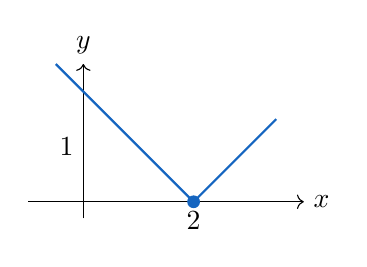
\begin{tikzpicture}[scale=0.7]
  \draw[->] (-1,0)--(4,0) node[right]{$x$};
  \draw[->] (0,-0.3)--(0,2.5) node[above]{$y$};
  \draw[thick,accentcolor] (-0.5,2.5)--(2,0)--(3.5,1.5);
  \filldraw[accentcolor] (2,0) circle(3pt);
  \node[below] at (2,0) {$2$};
  \node[left] at (0,1) {$1$};
\end{tikzpicture}
\end{center}
\end{answerbox}

\begin{notebox}
A function with a sharp corner (like $|x-a|$) is always continuous but not differentiable
at the corner point.
\end{notebox}

\vspace{4pt}

% ── Q3 ───────────────────────────────────────────────────────
\begin{questionbox}{3}{Applications of Derivatives — Local Extrema}{4}{CO2 / L4}
The function $f(x) = 2x^3 - 9x^2 + 12x - 4$ has a local \textbf{maximum} at:

\begin{enumerate}[label=(\Alph*), itemsep=4pt, topsep=6pt]
  \item $x = 1$
  \item $x = 2$
  \item $x = 3$
  \item $x = -1$
\end{enumerate}
\end{questionbox}

\begin{answerbox}{A}
\begin{align}
  f'(x) &= 6x^2 - 18x + 12 = 6(x^2 - 3x + 2) = 6(x-1)(x-2)
\end{align}
Critical points: $x = 1$ and $x = 2$.

\textbf{Second derivative test:}
\begin{align}
  f''(x) &= 12x - 18 \\
  f''(1) &= 12 - 18 = -6 < 0 \implies \text{local \textbf{maximum} at } \boxed{x = 1} \\
  f''(2) &= 24 - 18 = +6 > 0 \implies \text{local minimum at } x = 2
\end{align}
\end{answerbox}

\begin{notebox}
Second derivative test: $f''(c) < 0 \Rightarrow$ local max; $f''(c) > 0 \Rightarrow$ local min;
$f''(c) = 0 \Rightarrow$ test inconclusive (use first derivative test).
\end{notebox}

\vspace{4pt}

% ── Q4 ───────────────────────────────────────────────────────
\begin{questionbox}{4}{Definite Integrals}{4}{CO2 / L3}
The value of $\displaystyle\int_0^{\pi/2} \sin 2x\,dx$ is:

\begin{enumerate}[label=(\Alph*), itemsep=4pt, topsep=6pt]
  \item $0$
  \item $1$
  \item $\dfrac{\pi}{2}$
  \item $2$
\end{enumerate}
\end{questionbox}

\begin{answerbox}{B}
\begin{align}
  \int_0^{\pi/2} \sin 2x\,dx &= \left[-\frac{\cos 2x}{2}\right]_0^{\pi/2} \\[6pt]
  &= \left(-\frac{\cos\pi}{2}\right) - \left(-\frac{\cos 0}{2}\right) \\[6pt]
  &= \left(-\frac{-1}{2}\right) - \left(-\frac{1}{2}\right) \\[6pt]
  &= \frac{1}{2} + \frac{1}{2} = \boxed{1}
\end{align}
\end{answerbox}

\begin{notebox}
$\int \sin(ax)\,dx = -\dfrac{\cos(ax)}{a} + C$.
\quad
Property: $\displaystyle\int_0^{\pi/2} \sin^n x\,dx = \int_0^{\pi/2}\cos^n x\,dx$ (Wallis).
\end{notebox}

\vspace{4pt}

% ── Q5 ───────────────────────────────────────────────────────
\begin{questionbox}{5}{Differential Equations — Variable Separable}{4}{CO3 / L3}
The general solution of $\dfrac{dy}{dx} = \dfrac{y}{x}$ is:

\begin{enumerate}[label=(\Alph*), itemsep=4pt, topsep=6pt]
  \item $y = Cx^2$
  \item $y = Cx$
  \item $y = Ce^x$
  \item $y = \dfrac{C}{x}$
\end{enumerate}
\end{questionbox}

\begin{answerbox}{B}
Separating variables:
\begin{align}
  \frac{dy}{y} &= \frac{dx}{x}
\end{align}
Integrating both sides:
\begin{align}
  \ln|y| &= \ln|x| + \ln|C| \\
  \ln|y| &= \ln|Cx| \\
  y &= \boxed{Cx}
\end{align}
This represents a family of straight lines through the origin.
\end{answerbox}

\begin{notebox}
Variable separable form: $f(y)\,dy = g(x)\,dx$.
After integrating, always include the arbitrary constant $C$
(or $\ln C$ if using log form).
\end{notebox}

\vspace{4pt}

% ── Q6 ───────────────────────────────────────────────────────
\begin{questionbox}{6}{Vectors — Cross Product Magnitude}{4}{CO3 / L3}
If $\vec{a} = 2\hat{i} + 3\hat{j} - \hat{k}$ and $\vec{b} = \hat{i} - 2\hat{j} + 2\hat{k}$,
then $|\vec{a} \times \vec{b}|$ equals:

\begin{enumerate}[label=(\Alph*), itemsep=4pt, topsep=6pt]
  \item $\sqrt{195}$
  \item $\sqrt{90}$
  \item $\sqrt{179}$
  \item $\sqrt{150}$
\end{enumerate}
\end{questionbox}

\begin{answerbox}{B}
\[
  \vec{a} \times \vec{b} =
  \begin{vmatrix}
    \hat{i} & \hat{j} & \hat{k} \\
    2       & 3       & -1      \\
    1       & -2      & 2
  \end{vmatrix}
\]
\begin{align}
  &= \hat{i}\bigl(3 \cdot 2 - (-1)(-2)\bigr)
   - \hat{j}\bigl(2 \cdot 2 - (-1)(1)\bigr)
   + \hat{k}\bigl(2(-2) - 3 \cdot 1\bigr) \\
  &= \hat{i}(6-2) - \hat{j}(4+1) + \hat{k}(-4-3) \\
  &= 4\hat{i} - 5\hat{j} - 7\hat{k}
\end{align}
\[
  |\vec{a} \times \vec{b}| = \sqrt{4^2 + (-5)^2 + (-7)^2}
                           = \sqrt{16 + 25 + 49}
                           = \boxed{\sqrt{90} = 3\sqrt{10}}
\]
\end{answerbox}

\begin{notebox}
$|\vec{a} \times \vec{b}| = |\vec{a}||\vec{b}|\sin\theta$, where $\theta$ is the angle between them.
It also equals the area of the parallelogram formed by $\vec{a}$ and $\vec{b}$.
\end{notebox}

\vspace{4pt}

% ── Q7 ───────────────────────────────────────────────────────
\begin{questionbox}{7}{3D Geometry — Direction Cosines}{4}{CO4 / L3}
The angle $\theta$ between lines with direction cosines
$\left(\dfrac{1}{\sqrt{3}},\dfrac{1}{\sqrt{3}},\dfrac{1}{\sqrt{3}}\right)$
and $\left(\dfrac{1}{\sqrt{2}},\dfrac{1}{\sqrt{2}},0\right)$ is:

\begin{enumerate}[label=(\Alph*), itemsep=4pt, topsep=6pt]
  \item $90^\circ$
  \item $60^\circ$
  \item $45^\circ$
  \item $\cos^{-1}\!\left(\dfrac{2}{\sqrt{6}}\right)$
\end{enumerate}
\end{questionbox}

\begin{answerbox}{D}
\begin{align}
  \cos\theta &= l_1 l_2 + m_1 m_2 + n_1 n_2 \\
             &= \frac{1}{\sqrt{3}}\cdot\frac{1}{\sqrt{2}}
              + \frac{1}{\sqrt{3}}\cdot\frac{1}{\sqrt{2}}
              + \frac{1}{\sqrt{3}}\cdot 0 \\
             &= \frac{1}{\sqrt{6}} + \frac{1}{\sqrt{6}} + 0
              = \frac{2}{\sqrt{6}}
\end{align}
\[
  \theta = \boxed{\cos^{-1}\!\left(\frac{2}{\sqrt{6}}\right) \approx 35.26^\circ}
\]
\end{answerbox}

\begin{notebox}
For direction cosines $(l,m,n)$: $l^2+m^2+n^2=1$.
\quad
Two lines are perpendicular iff $l_1 l_2 + m_1 m_2 + n_1 n_2 = 0$.
\end{notebox}

\vspace{4pt}

% ── Q8 ───────────────────────────────────────────────────────
\begin{questionbox}{8}{Probability — Without Replacement}{4}{CO4 / L3}
Two cards are drawn \textbf{without replacement} from a standard deck of 52 cards.
The probability that \textbf{both} are aces is:

\begin{enumerate}[label=(\Alph*), itemsep=4pt, topsep=6pt]
  \item $\dfrac{1}{221}$
  \item $\dfrac{1}{169}$
  \item $\dfrac{4}{52}$
  \item $\dfrac{1}{26}$
\end{enumerate}
\end{questionbox}

\begin{answerbox}{A}
\begin{align}
  P(\text{both aces}) &= P(\text{1st ace}) \times P(\text{2nd ace} \mid \text{1st ace}) \\[6pt]
                      &= \frac{4}{52} \times \frac{3}{51} \\[6pt]
                      &= \frac{12}{2652} = \boxed{\frac{1}{221}}
\end{align}
\end{answerbox}

\begin{notebox}
With replacement: $P = \dfrac{4}{52} \times \dfrac{4}{52} = \dfrac{1}{169}$.\quad
Without replacement: $P = \dfrac{4}{52} \times \dfrac{3}{51} = \dfrac{1}{221}$.
The distinction matters whenever sampling is sequential.
\end{notebox}

\vspace{4pt}

% ── Q9 ───────────────────────────────────────────────────────
\begin{questionbox}{9}{Relations \& Functions}{4}{CO1 / L4}
The function $f : \mathbb{R} \to \mathbb{R}$ defined by $f(x) = x^2$ is:

\begin{enumerate}[label=(\Alph*), itemsep=4pt, topsep=6pt]
  \item One-one and onto
  \item One-one but not onto
  \item Onto but not one-one
  \item Neither one-one nor onto
\end{enumerate}
\end{questionbox}

\begin{answerbox}{D}
\textbf{One-one (injective)?} No.
$f(2) = 4 = f(-2)$ but $2 \neq -2$. \quad$\therefore$ \textit{not} injective.

\textbf{Onto (surjective)?} No.
For $y = -1 \in \mathbb{R}$, there is no $x \in \mathbb{R}$ such that $x^2 = -1$. \quad$\therefore$ \textit{not} surjective.

$\boxed{\text{Neither one-one nor onto}}$

\smallskip
\textit{Note:} $f : \mathbb{R} \to [0,\infty)$ would make it surjective; $f:[0,\infty)\to[0,\infty)$ makes it bijective.
\end{answerbox}

\begin{notebox}
Domain and codomain matter.
$f(x)=x^2$ with domain $\mathbb{R}$ and codomain $\mathbb{R}$: neither injective nor surjective.
Restricting to $[0,\infty)\to[0,\infty)$: bijective.
\end{notebox}

\vspace{4pt}

% ── Q10 ──────────────────────────────────────────────────────
\begin{questionbox}{10}{Inverse Trigonometry — Compound Angles}{4}{CO1 / L3}
The value of $\sin\!\left(\tan^{-1}\dfrac{3}{4} + \tan^{-1}\dfrac{5}{12}\right)$ is:

\begin{enumerate}[label=(\Alph*), itemsep=4pt, topsep=6pt]
  \item $\dfrac{33}{65}$
  \item $\dfrac{56}{65}$
  \item $\dfrac{63}{65}$
  \item $\dfrac{16}{65}$
\end{enumerate}
\end{questionbox}

\begin{answerbox}{B}
Let $\alpha = \tan^{-1}\!\dfrac{3}{4}$ and $\beta = \tan^{-1}\!\dfrac{5}{12}$.

From a right triangle: $\sin\alpha = \dfrac{3}{5}$, $\cos\alpha = \dfrac{4}{5}$;
$\;\sin\beta = \dfrac{5}{13}$, $\cos\beta = \dfrac{12}{13}$.

Using the compound angle formula:
\begin{align}
  \sin(\alpha+\beta) &= \sin\alpha\cos\beta + \cos\alpha\sin\beta \\
                     &= \frac{3}{5}\cdot\frac{12}{13} + \frac{4}{5}\cdot\frac{5}{13} \\
                     &= \frac{36}{65} + \frac{20}{65} = \boxed{\dfrac{56}{65}}
\end{align}
\end{answerbox}

\begin{notebox}
For $\tan^{-1}(a/b)$: draw a right triangle with opposite $= a$, adjacent $= b$,
hypotenuse $= \sqrt{a^2+b^2}$, then read off $\sin$ and $\cos$ directly.
\end{notebox}

\label{LastPage}
\end{document}
